\chapter{Grundlagen}
\section{Ultraschall}
\subsection{Definition}
Schallwellen sind mechanische Wellen. Dabei unterscheidet man Infraschall\footnote{Frequenzen $< 20$ Hz}, Ultraschall\footnote{Frequenzen $>20.000$ Hz \ac{bzw} 20 kHz} und Schallwellen, welche das menschliche Gehör wahrnehmen kann\footnote{Frequenzen von 20 bis 20.000 Hz}.
\begin{figure}[h]
		\centering
  		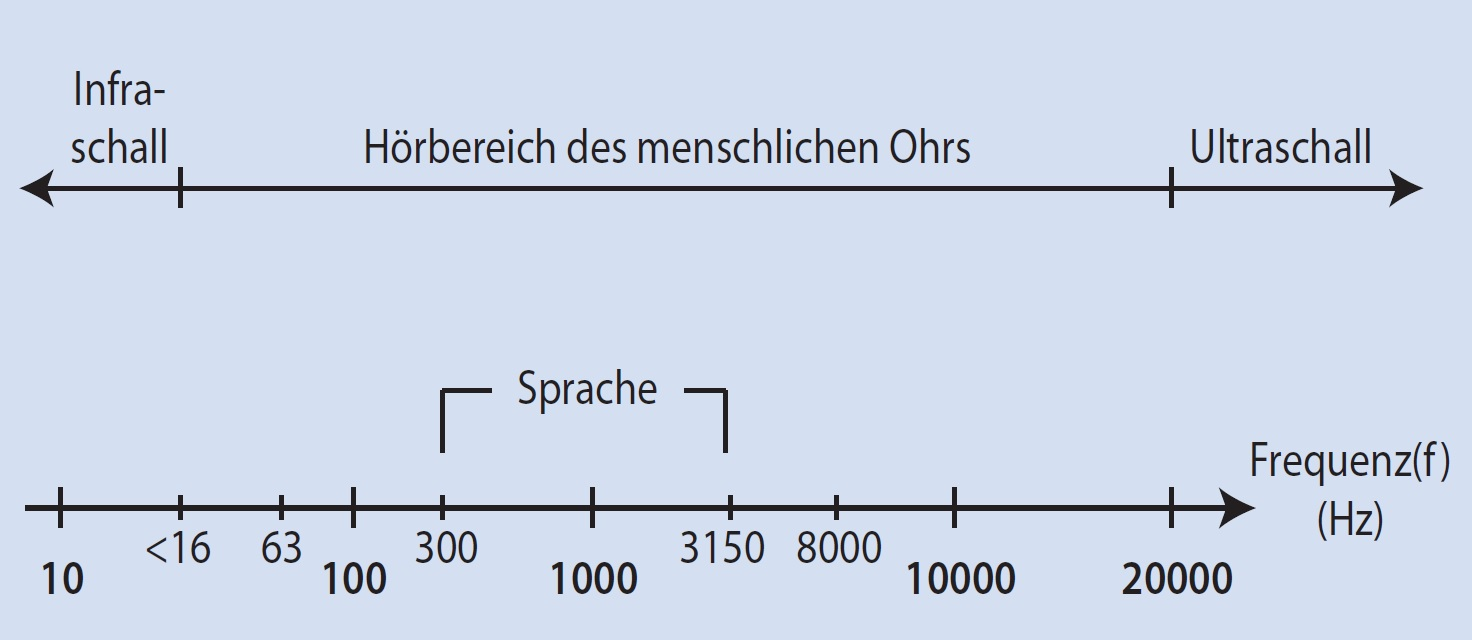
\includegraphics[trim = 0cm 0.5cm 0cm 1.5cm, clip=true, width=\textwidth]{Schall}  
  		\caption{Frequenzbereiche Schall}
  		\label{fig:Schall}
  	\end{figure}
Die höchsten, technisch realisierbaren Schallfrequenzen liegen bei \ac{ca} 1 \ac{ghz}. Für die medizinische Diagnostik sind dabei Frequenzen im Bereich von 2 bis 10 \ac{mhz} interessant. Unterhalb von 2 \ac{mhz} ist die Auflösung zu gering und oberhalb von \ac{ca} 10 \ac{mhz} ist die Absorption im Gewebe zu stark.\newline
In menschlichem Gewebe beträgt die Schallgeschwindigkeit $c$ etwa 1500 $m/s$. Bei Frequenzen im Bereich von 2 bis 10 \ac{mhz} ist deshalb die Wellenlänge $\lambda$ im Bereich von $<$ 10 mm. Somit kann man erreichen, dass sich Ultraschall im Gewebe wie ein optischer Strahl ausbreitet. Er kann fokussiert, reflektiert, gestreut und absorbiert werden. Durch diese Effekte kann somit eine Abbildung von Organen erzielt werden, welche die Basis der Sonographie oder Ultraschalldiagnostik bildet.%
\cite{suter2006}\cite{suter2009}\cite{suter2010}
%
\subsection{Erzeugung und Empfang}
Im Jahr 1880 wurde der \textit{Piezoelektrische Effekt} von Pierre Curie entdeckt. Der Effekt bezieht sich auf Materialien, welche einen permanenten elektrischen Dipolmoment\footnote{Materialien, bei denen die Schwerpunkte der positiven und negativen Ladungen nicht zusammenfallen} aufweisen. Diese erzeugen eine Spannung, wenn eine Kraft (\ac{resp} ein Druck) angelegt wird.\\
Mit diesem Effekt ist es möglich Kräfte, jedoch aber auch Torsion oder wie in dieser Arbeit Ultraschall zu messen. 
\begin{figure}[hb]
	\centering
	\begin{subfigure}[b]{0.49\textwidth}
		\centering
  		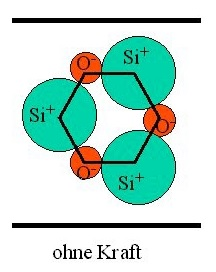
\includegraphics[trim = 0mm 10mm 0mm 0mm, clip, scale=0.5]{Piezo_without}  
  		\caption{ohne Kraft}
  		\label{fig:piezo_without}
  	\end{subfigure}
  	\hfill
  	\begin{subfigure}[b]{0.49\textwidth}
	  	\centering
  		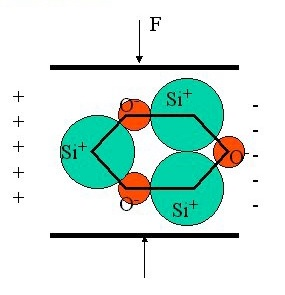
\includegraphics[trim = 0mm 10mm 0mm 0mm, clip, scale=0.5]{Piezo_with}  
  		\caption{Ein Druck erzeugt eine Kraft}
  		\label{fig:piezo_with}
  	\end{subfigure}
  	\caption{Piezoelektrischer Effekt}
  	\label{fig:piezo}
\end{figure}
Dieser Effekt kann aber auch zur Erzeugung von Kraft in Form von mechanischen Wellen genutzt werden. Dies bezeichnet man als den \textit{Indirekten piezoelektrischen Effekt}. Durch Anlegen einer Wechselspannung an einen elastischen Körper wird dieser mit der Frequenz der Wechselspannung verformt und erzeugt in Abhängigkeit der Körpereigenschaften, der Amplitude der angelegten Wechselspannung und deren Frequenz Schallwellen.
%
\cite{suter2006}\cite{suter2009}\cite{suter2010}
%
\subsection{Ausbreitung}\label{sec:ausbreitung}
Eine Schallwelle entspricht einer zeitlichen und räumlichen periodischen Auslenkung von Druck und Dichte des Mediums. Dabei interessieren vor allem die Änderungen des Drucks (nicht der Mittelwert). Somit sind Schallwellen an Materie gebunden und können sich im Vakuum nicht ausbreiten. In Luft, Flüssigkeiten sowie biologischen Gewebe breiten sich Schallwellen dabei in Form von Longitudinalwellen\footnote{von Zonen mit Über- und Unterdruck (Verdichtungs- und Verdünnungszonen)} aus. \\
Dabei hängt die Schallgeschwindigkeit $c$ in Festkörpern von der Dichte \(\rho\), der Poissonzahl \(\mu\) und dem Elastizitätsmodul \(E\) ab. Es ist dabei die Schallgeschwindigkeit $c$ im Festkörper:
\begin{equation}
c_{longitudinal}=\sqrt{\dfrac{E(1-\mu)}{\rho(1-\mu-2\mu^2)}}\label{eq:c_long}
\end{equation}
\begin{equation}
c_{transversal}=\sqrt{\dfrac{E}{2\rho(1+\mu)}}\label{eq:c_trans}
\end{equation}
Mit der \autoref{eq:c_long} werden für die Medizin wichtigen Schallgeschwindigkeiten für die aufgeführten Materialien bestimmt (siehe \autoref{tab:Schallgeschwindigkeiten}).
Der Schalldruck und die Schallimpedanz darf dabei nicht vernachlässigt werden, da die Ausbreitung von Druck und Dichte des Mediums abhängig ist.\\
Für die Schallimpedanz $Z$ findet man:
\begin{equation}
Z=\dfrac{\Delta\rho_0}{\upsilon_0}=\sqrt{K\cdot\rho_0}
\label{eq:z over rho}
\end{equation}
\begin{equation}
Z=c\cdot\rho
\label{eq:z over c}
\end{equation}
Aus den Gleichungen \ref{eq:z over rho} und \ref{eq:z over c} ist erkennbar, dass die Schallimpedanz $Z$ eine Materialkonstante ist.\newline
Die Intensität einer Schallschwelle\footnote{Energietransport pro Fläche und Zeiteinheit} ist
\begin{equation}
j=\dfrac{\text{Kraft $\cdot$ Weg}}{\text{Fläche $\cdot$ Zeit}}=\rho\cdot c
\label{eq:j}
\end{equation}
Mit der kinetischen Energiedichte \(\rho v^2\) kann die Schallintensität auch ausgedrückt werden durch
\begin{equation}
j=\rho c v^2
\end{equation}
In Bezug auf die Zeit ist sie damit
\begin{equation}
j=\rho_0 c A_0^2\omega^2 sin^2(\omega t)
\end{equation}
wobei die Amplitude \(A_0\) die Auslenkung \(A_0 sin(\omega t)\) darstellt.
%
\cite{suter2006}\cite{suter2009}\cite{suter2010}
%
\subsection{Reflexion und Brechung}\label{sec:schall_reflection}
Wie alle Wellen werden auch Schallwellen an Grenzflächen teilweise reflektiert. Diese Grenzflächen befinden sich zwischen Gebieten mit unterschiedlicher Schallimpedanz.
Bei senkrechtem Einfall im linearen Bereich gilt für die transmittierte Intensität $I_t$ mit der emittierten Intensität $I_e$
\begin{equation}
\frac{I_t}{I_e}=4\dfrac{Z_1Z_2}{(Z_1+Z_2)^2}
\end{equation}
und für die Intensität der reflektierten Welle $I_r$
\begin{equation}
\frac{I_r}{I_e}=\dfrac{(Z_1-Z_2)^2}{(Z_1+Z_2)^2}
\label{eq:i of reflection}
\end{equation}
Da in der Sonographie hauptsächlich mit den reflektierten Wellen gearbeitet wird, beziehen sich die nächsten Aussagen auf die \autoref{eq:i of reflection}. Unter Betrachtung der \autoref{tab:Schallgeschwindigkeiten}  und der \autoref{eq:z over c} erschließt sich, dass die Schallimpedanzen der biologischen Materialien sehr gering sind. Somit kann \autoref{eq:i of reflection} weiter vereinfacht und der Reflektionsfaktor $R$ bestimmt werden.
\begin{equation}
R\approx \dfrac{\left(\Delta Z\right)^2}{4Z^2}
\end{equation}
Hingegen ist der Reflektionsfaktor zwischen Luft und dem biologischen Gewebe extrem groß und reduziert die Intensität dementsprechend stark. Diesem Effekt muss durch ein spezielles Kontaktgel entgegengewirkt werden.
%
\cite{suter2006}\cite{suter2009}\cite{suter2010}
%
\subsection{Absorption und Streuung}
Wie in \autoref{sec:schall_reflection} dargestellt nimmt die Gesamtintensität der Ultraschallwelle bei jeder Grenzfläche ab. Zudem wird das Medium durch die einstrahlende Welle in Schwingung versetzt und strahlt somit selbst eine Welle aus. \\
Findet diese Schwingung in Phase mit der einfallenden Welle statt\footnote{homogenes Medium}, beeinflusst die Interferenz zwischen den Wellen lediglich die Phasengeschwindigkeit der Ultraschallwelle.\\
Eine Überlagerung der Wellen hingegen\footnote{in inhomogenen Medium} führt zu einer Schallabstrahlung in alle Richtungen und somit zu einer Streuung, was eine Dämpfung zu Folge hat.\newline
Da das biologische Gewebe jedoch eher einem homogenen Medium entspricht, ist die Abnahme für eine ebene Welle proportional zur Intensität und nimmt somit exponentiell ab
\begin{equation}
I(x)=I_0e^{-\mu x}
\end{equation}
Dabei besteht der Dämpfungs- oder Schwächungskoeffizient $\mu$ aus einem Absorptions- und einem Streuanteil \(\mu = \mu_{Abs}+\mu_{Streu}\). Im Gewebe beträgt die Dämpfung \ac{ca} $1\dfrac{dB}{cm\ \ac{mhz}}$ 
Die Effizienz der Streuung hängt von der Frequenz / Wellenlänge $\lambda$, der Größe der streuenden Inhomogenitäten und dem Unterschied der Schallimpedanz ab. \\
Streuung und Absorption bestimmen zusammen die Eindringtiefe der Schallwellen.
Somit ist die Dämpfung abhängig von dem \textbf{Koeffizienten \(\mu\)}, dem \textbf{Weg \(x\)} und der \textbf{Sendefrequenz \(f\)}.
%
\cite{suter2006}\cite{suter2009}\cite{suter2010}
%
\subsection{Dopplereffekt}\label{sec:dopplereffekt}
Der Effekt tritt bei allen mechanischen Wellen auf, die sich durch den Raum bewegen. Dabei erregt die Welle stationäre und sich bewegende Teilchen gleichermaßen, wodurch eine weitere Welle durch das erregte Teilchen ausgesendet wird. Bei stationären Teilchen wird die Trägerfrequenz $f_0$ reflektiert. Die bewegenden Teilchen jedoch führen je nach Bewegungsrichtung zur Welle kinetische Energie zu der Reflektion der Welle hinzu oder ab\footnote{Teilchen können beschleunigt oder abgebremst werden}. Bewegt sich ein Teilchen entgegen der Longitudinalwellenrichtung so wird die reflektierte Wellenlänge $\lambda$ größer. Umgekehrt wird $\lambda$ kleiner, wenn sich ein Teilchen mit der Longitudinalwellenrichtung bewegt.\newline
Die Differenz $\Delta f$ zwischen emittierter und empfangener Trägerfrequenz nennt man Dopplerschiebefrequenz. Die Differenz ist abhängig von der Trägerfrequenz $f$ und dem Geschwindigkeitsvektor $\overrightarrow{v}$ des bewegten Teilchens. Somit ist der Winkel $\theta$ zwischen Ausbreitungsrichtung der Welle und des Richtungsvektors des Teilchens nicht vernachlässigbar.\\
Die Dopplerschiebefrequenz berechnet sich nach folgender Gleichung
\begin{equation}
\Delta f=\dfrac{2fv\ cos(\theta)}{c}
\end{equation}
Anwendung findet dieser Effekt nicht nur in der diagnostischen Medizin zur Bestimmung von Blutströmungsgeschwindigkeiten. Der Effekt dient seit Jahren in der Industrie und in Haushalten zur Überwachung des Durchflussvolumens und der Erkennung von Fremdkörpern in Flüssigkeiten. Die Dopplerschiebefrequenzen liegen dabei in der diagnostischen Medizin im hörbaren Bereich von einigen kHz.

\section{\acl{pw} Dopplerverfahren}\label{sec:pw}
Beim gepulsten Dopperverfahren werden Bursts\footnote{kurz-gepulste Energiepakete} durch den Transduktor in Kombination mit einen Piezoelement erzeugt. Diese werden in periodischen Abständen (\acf{prf}) in das zu messende Material transmittiert. Dabei werden durch Teilchen oder Dichteänderungen Reflexionen verursacht (\autoref{sec:schall_reflection}), welche mit demselben Piezoelement erfasst und anhand der Laufzeit (\autoref{sec:ausbreitung}) bestimmten Materialtiefen zugeordnet werden kann.\\
Statische Reflexionen verursachen dabei stärkere Signale als die dynamischen Dopplersignale und müssen nachträglich aus der Messung gefiltert werden. Dies geschieht durch die sogenannte Demodulation.\\
\autoref{fig:pw_timing} visualisiert den Ereignisablauf für zwei überlagerte Messtiefen in Abhängigkeit der Peripherieansteuerung. Dabei wird die \ac{prf} durch den Impuls \textit{Retransmit} realisiert, welches die Erzeugung des Burstsignals zur Folge hat. Anschließend werden durch die Zeitdifferenzen, die zu messenden Tiefenbereiche digitalisiert sowie demoduliert. Dabei wird für jeden Tiefenbereich bzw. für jede \ac{roi} eine bestimmte Anzahl von Messwerten generiert und zusammengefasst.\\
\definecolor{fgblue}{rgb}{0,0,0.6}%
\definecolor{fgred}{rgb}{0.6,0,0}%
\begin{figure}[h!]
\centering
\begin{tikztimingtable}
[timing/d/background/.style={fill=white},
timing/c/.cd]
Clock 			& 185{0.2C} \\
\acs{prf} 			& D{}35D{}D{} \\
BURST 			& [fgblue] L 10{0.1H 0.1L} 33L 5{0.1H 0.1L} \\
ADC				& [fgblue] 5L 30H 2L \\
\ac{roi} 1 	& [fgred] 5L 10{2D{}} 12L \\
\ac{roi} 2 	& [fgred] 15L 10{2D{}} 2L \\
Retransmit		& L G 35L G L \\
\extracode
	\draw (0 ,0) circle (0.5 pt); % Origin
	\begin{pgfonlayer}{background}
		\vertlines [help lines]{1,3,5,15,25,35,36}
	\end{pgfonlayer}
%	\tablegrid
\end{tikztimingtable}
\caption{Ereignis-Zeitdiagramm}
\label{fig:pw_timing}
\end{figure}
\hfill
\begin{table}[h!t]
\centering
\caption{Schallgeschwindigkeiten in unterschiedlichen Materialien und Geweben}
\label{tab:Schallgeschwindigkeiten}
\begin{tabular}{l|r}
\textbf{Material} & \textbf{c $\left[\frac{m}{s}\right]$} \\
\cline{1-2}
Luft 				  & $340$	 \\ 
Fett 				  & $1400$	 \\ 
Wasser $(37^\circ C)$ & $1540$	 \\ 
Leber 				  & $1549$ 	 \\ 
Niere 				  & $1561$ 	 \\ 
Muskel 				  & $1568$ 	 \\ 
Blut 				  & $1570$ 	 \\ 
Knochen 			  & $3600$ 	 \\ 
\end{tabular}
\end{table}
\begin{table}[h!t]
\centering
\caption{Eindringtiefen als Funktion der Frequenz in menschlichen Geweben}
\label{tab:Eindringtiefen}
\begin{tabular}{l|l|l}
\textbf{Frequenz f in $\ac{mhz}$} & \textbf{Eindringtiefe in $cm$} & \textbf{Anwendung} \\
\cline{1-3}
1 	& 50	& 	 \\ 
3.5 & 15	& Fötus, Leber, Herz, Niere	 \\ 
5 	& 10	& Gehirn \\ 
7.5 & 7 	& Prostata \\ 
10 	& 5 	& Pankreas \\ 
20 	& 1.2 	& Auge, Haut \\ 
40 	& 0.6 	& Intravaskulär \\ 
\end{tabular}
\end{table}